\def\year{2015}
%File: formatting-instruction.tex
\documentclass[letterpaper]{article}
\usepackage{aaai}
\usepackage{times}
\usepackage{helvet}
\usepackage{courier}
\usepackage{graphicx} % support the \includegraphics command and options
\usepackage{subcaption}
\frenchspacing
\setlength{\pdfpagewidth}{8.5in}
\setlength{\pdfpageheight}{11in}
\pdfinfo{
/Title (Insert Your Title Here)
/Author (Put All Your Authors Here, Separated by Commas)}
\setcounter{secnumdepth}{0}  
\begin{document}

We have devised several, two-agent grid world games that require differing levels of coordination, and also allow agents to defend against uncooperative partners. Each agent chooses one of five actions (north, south, east, west, wait), which are then executed simultaneously. Agent transition dynamics are deterministic, and there is no tie-breaking when two agents collide. Instead both agents remain on their current location if their chosen actions would collide with one another.


Figure~\ref{fig:fivebyfivehardwalls} is the simplest example of a coordinating grid game. The two agents moving toward their own goals should not interfere with one another. However, a very competitive agent might choose to interfere with the other agent's actions sacrificing their own best-path.

\begin{figure}
\centering
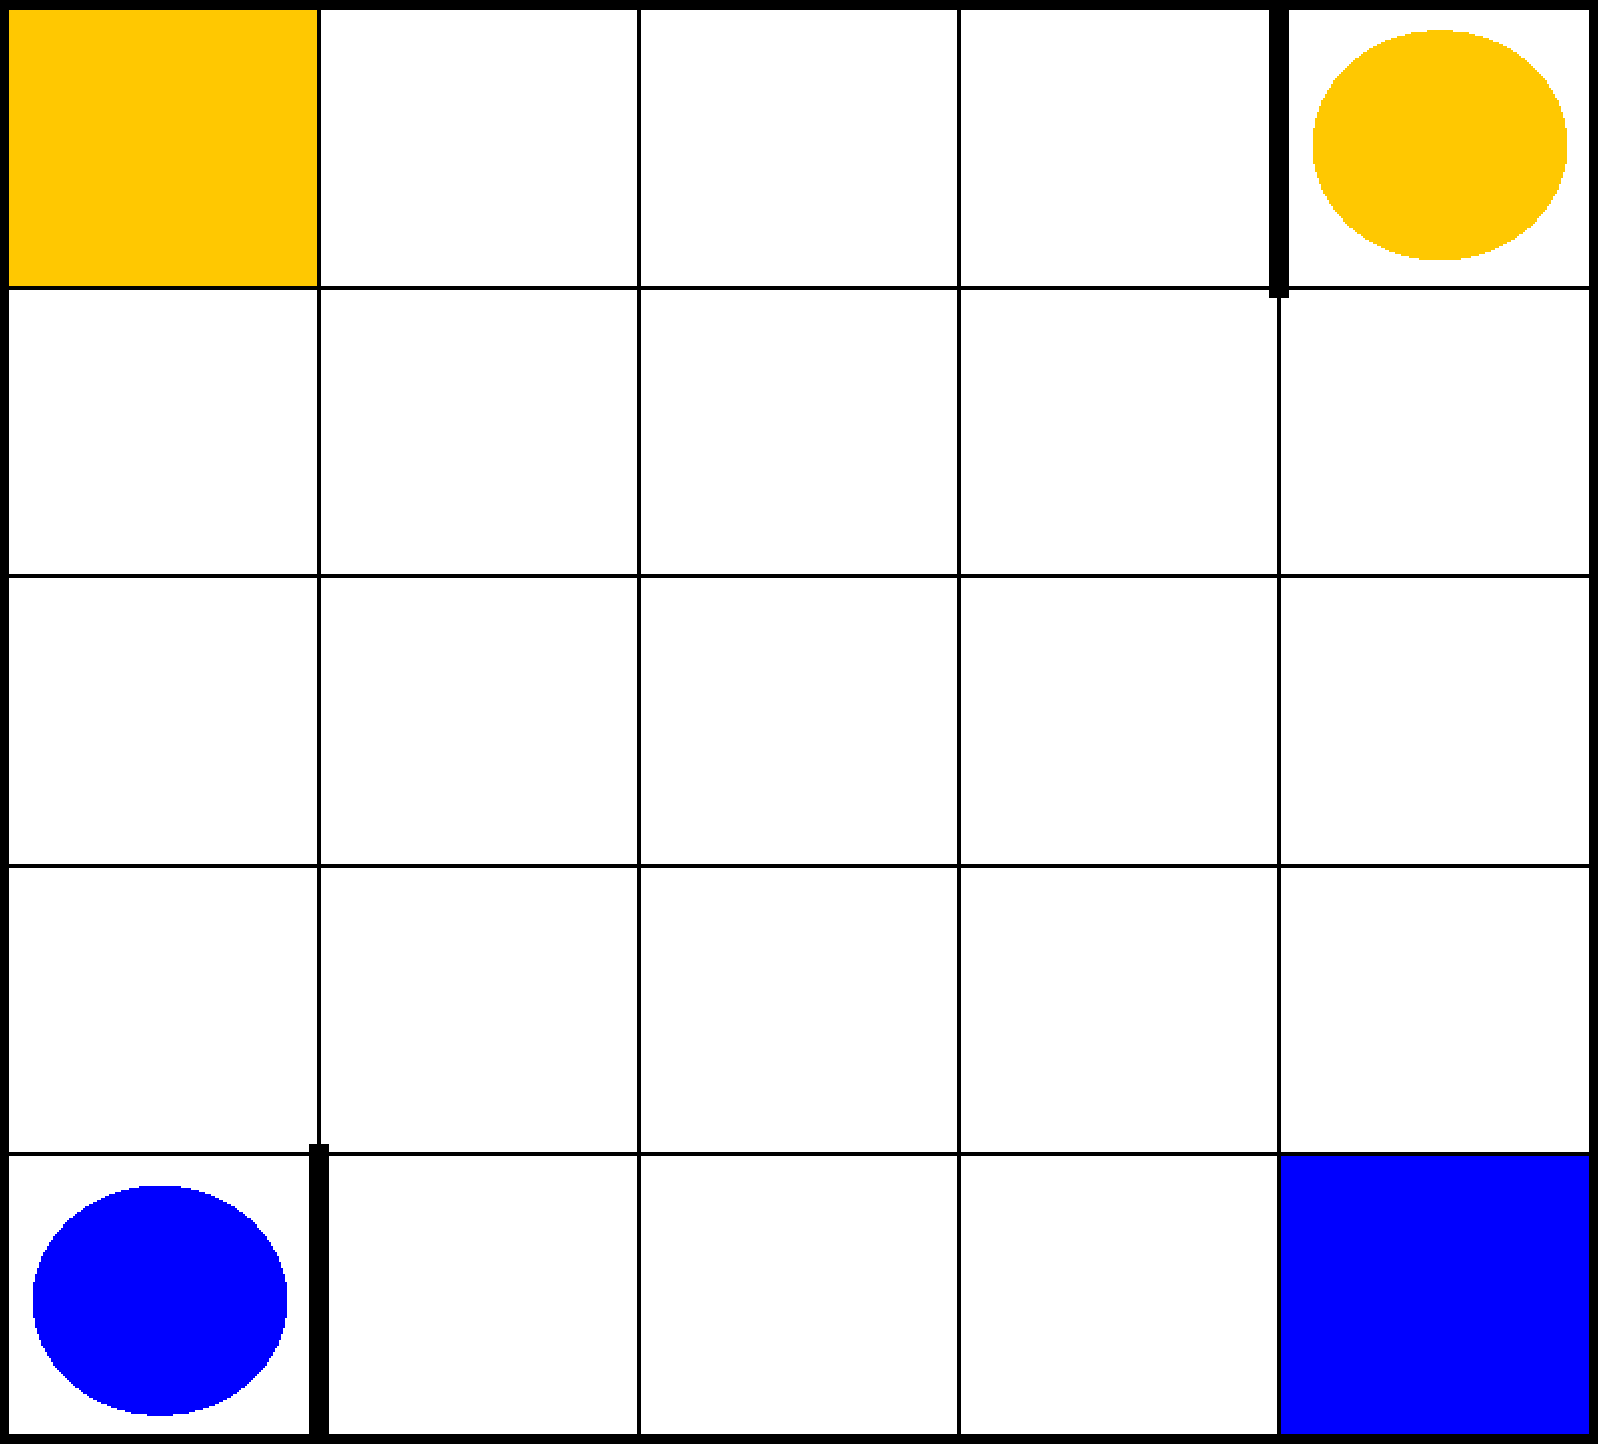
\includegraphics[width=0.8\columnwidth]{figures/fivebyfivehardwalls.png}
\caption{Five by five grid world require minimum coordination between the agents to reach the goals simultaneously}
\label{fig:fivebyfivehardwalls}
\end{figure}

The game in figure~\ref{fig:fivebyfivenowalls} requires coordinating for both agents to achieve a best-path toward their goals, which do not interfere with one another. After initial repetitions of the game, there is no motivation for either agent to deviate from the agreed upon strategy.

\begin{figure}
\centering
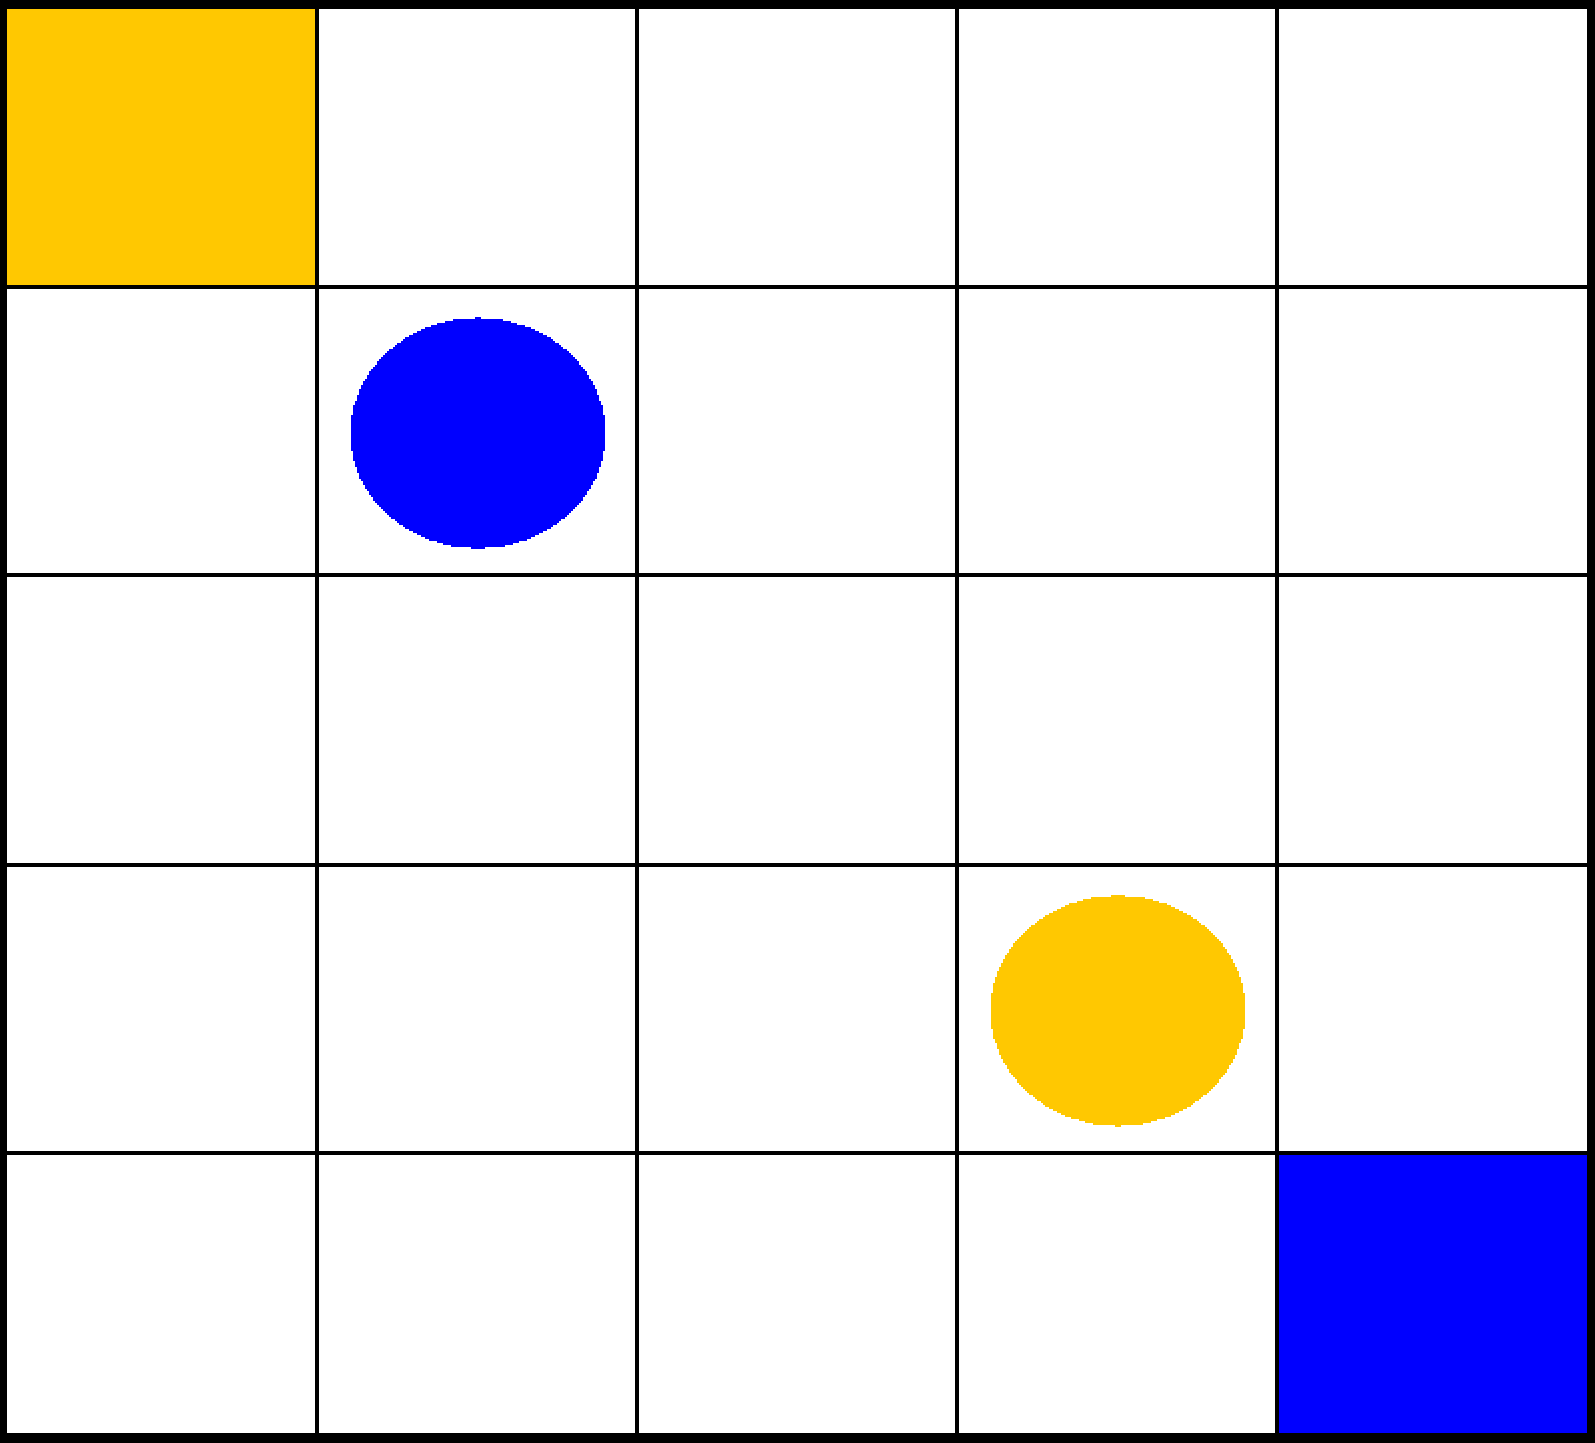
\includegraphics[width=0.8\columnwidth]{figures/fivebyfivenowalls.png}
\caption{Five by five grid world, which requires choosing a best-path that does not interfere with the other agent.}
\label{fig:fivebyfivenowalls}
\end{figure}

The grid world shown in figure~\ref{fig:fivebyfivesemiwalls} includes a semi-wall. There is a 50\% chance an agent that an agent who chooses to pass through it will succeed. The expected number of turns to proceed from the starting position, through the semi-wall to the goal is 5, but a longer deterministic route of 6 steps exists for two coordinating agents. Two agents that both choose to walk through the semiwalls will lose one-third of the time reducing the utility for not coordinating. However an agent that chooses to defect and attempt to walk through the semi-wall while the other agent trusts and pursues the longer route will win 50\%, tie 25\%, and lose 25\% of the time.

\begin{figure}
\centering
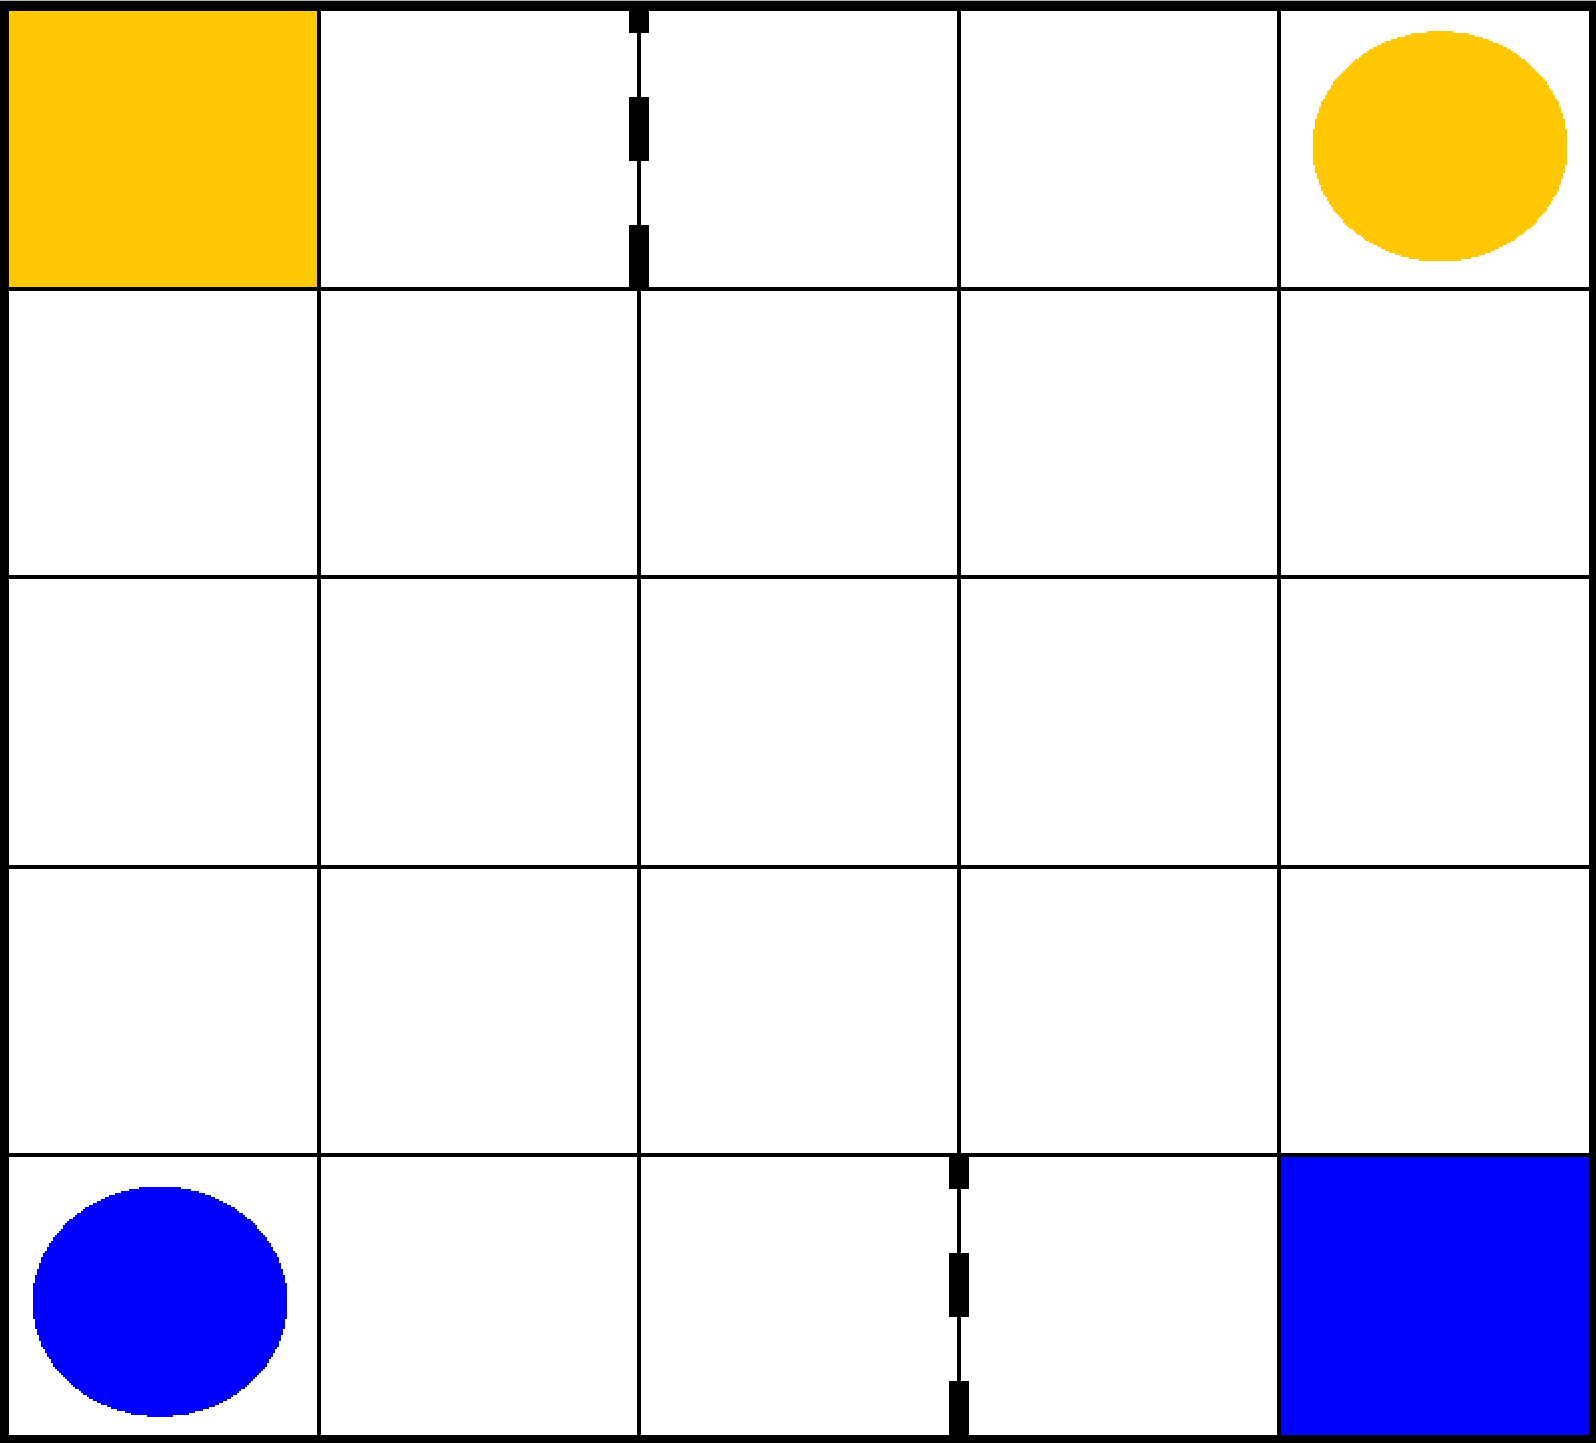
\includegraphics[width=0.8\columnwidth]{figures/fivebyfivesemiwalls.png}
\caption{Five by five grid world with walls that have 50-50 chance of passing through each try. Coordination requires sacrificing the best path for a concrete path that allows both agents to reach the goal simultaneously}
\label{fig:fivebyfivesemiwalls}
\end{figure}

The grid world in figure~\ref{fig:fivebyfivewalls} requires coordinating which agent is to go down which corridor. However, before a coordinating strategy has been agreed upon, two agents which pass into the same corridor, must negotiate a coordination that allows both to reach their goals. An agent that attempts to reverse course and go back to the other corridor will lose. Instead, one agent must defend and squat on the other's goal in that corridor to allow the agent to pass by so they both can reach their goal simultaneously.	

\begin{figure}
\centering
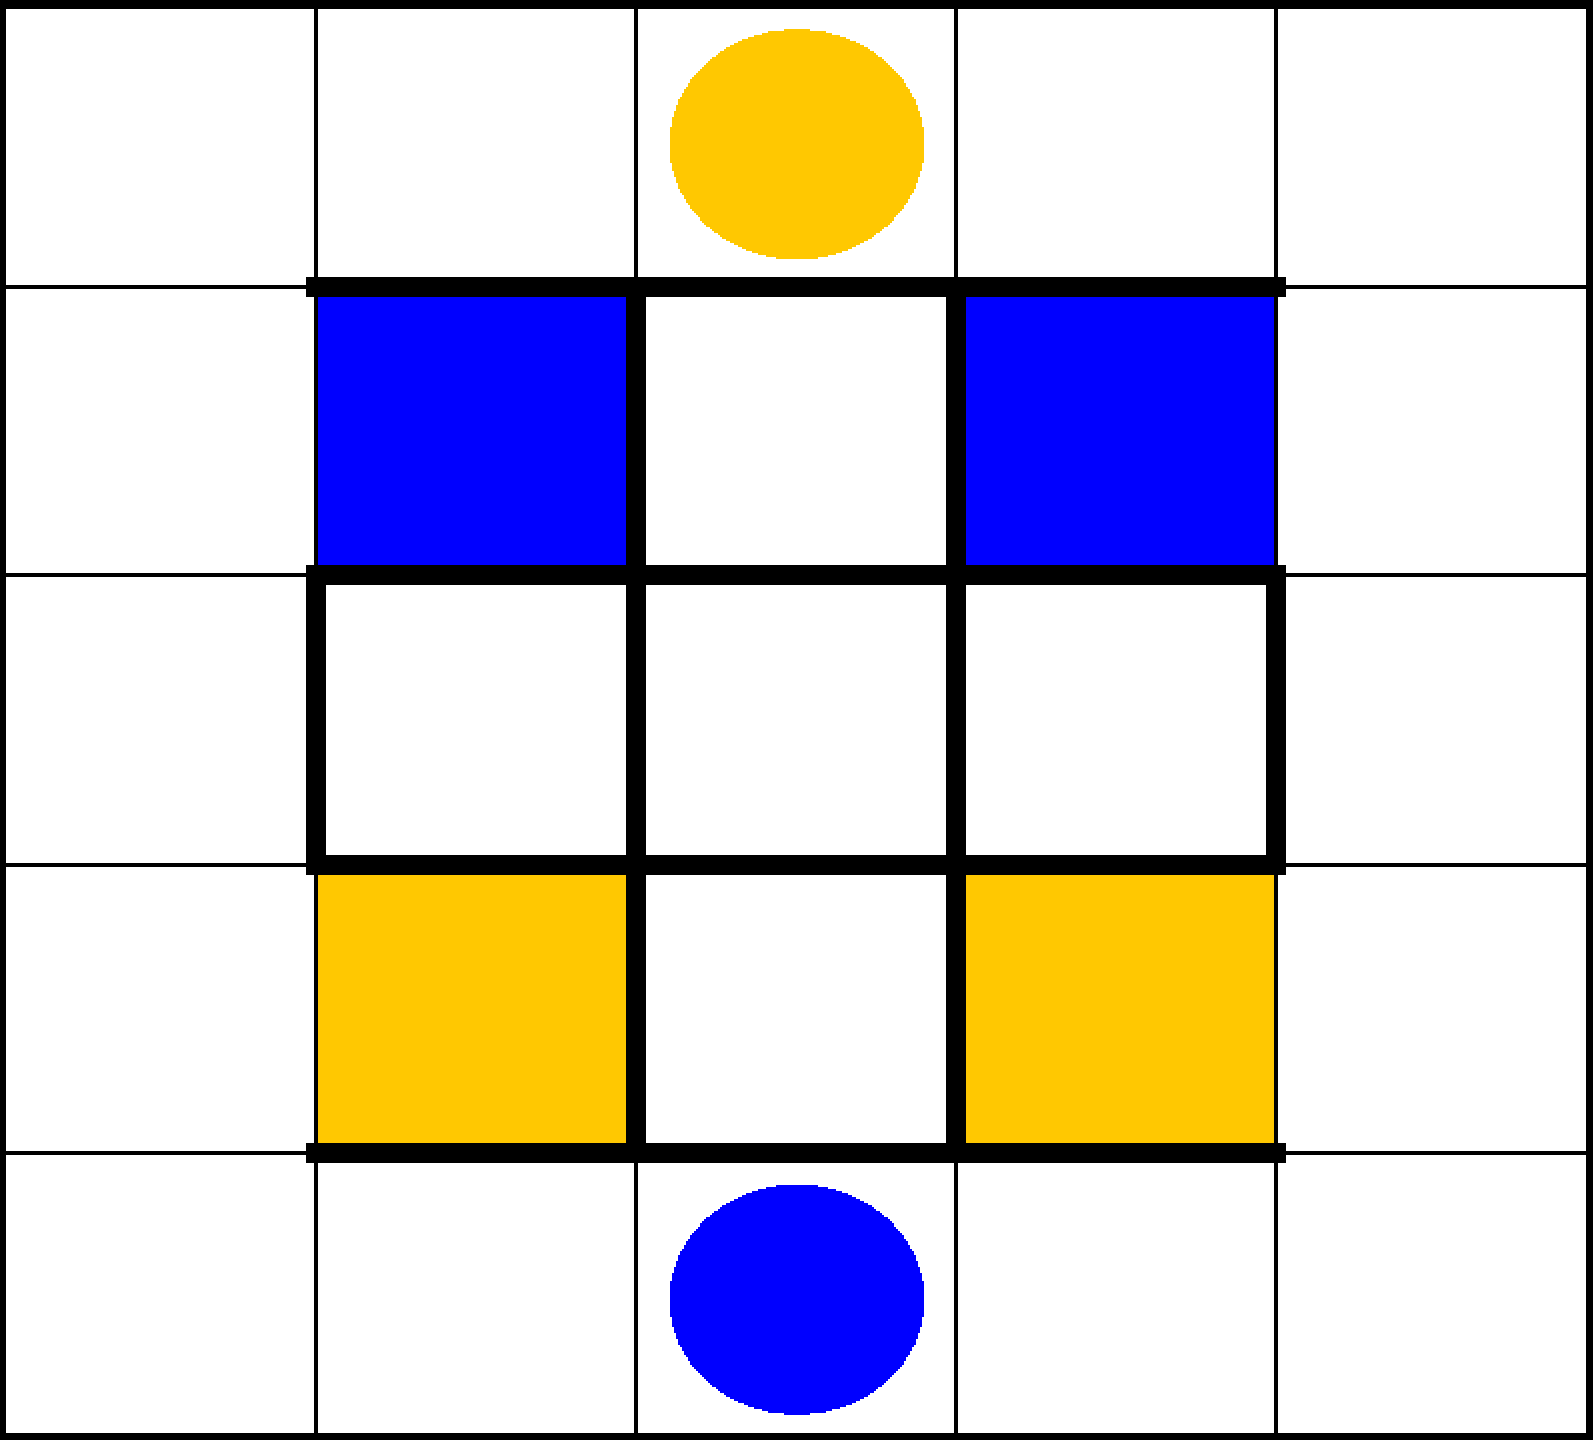
\includegraphics[width=0.8\columnwidth]{figures/fivebyfivewalls.png}
\caption{Five by five grid with many walls, which require each agent to agree on a cooridor, or coordinate should they choose the some one.}
\label{fig:fivebyfivewalls}
\end{figure}

The three by five grid world in figure~\ref{fig:threebyfivetwowalls} and figure~\ref{fig:threebyfive} allows both agents to coordinate through a trusting strategy where one agent moves along the high road and the other along the low road without interfering with one another. However, an agent which notices the other is trusting might choose on the next game iteration to defect and proceed straight to the goal. There are strategies to defend against an non-cooperative agent. For example if the orange agent moves north initially to $(1,3)$ and blue moves to $(4,2)$, the orange agent might choose to return and remain on its goal before the blue agent moves to $(4,3)$, where they are then equidistant from their goals. A more explicit defensive strategy for the orange agent would have it proceed to $(2,3)$, and then choose to move south to $(2,2)$. If the blue agent is in $(3,2)$ and attempting to move west into $(2,2$), they would collide until one agent chooses a different action. It would be in orange's best interest to continue choosing the south action to go into $(2,2)$ and wait until blue surrenders and chooses to go south into $(2,0)$ or north into $(2,2)$. They are then equidistant and can proceed to their respective goals. This strategy, which we call \textit{cooperative-defensive}, allows each agent to choose a mutually agreeable strategy while also defending against an agent that is uncooperative. Figure~\ref{fig:threebyfivetwowalls} implies a direction for each agent's coordination, while figure~\ref{fig:threebyfive} does not.

\begin{figure}
\centering
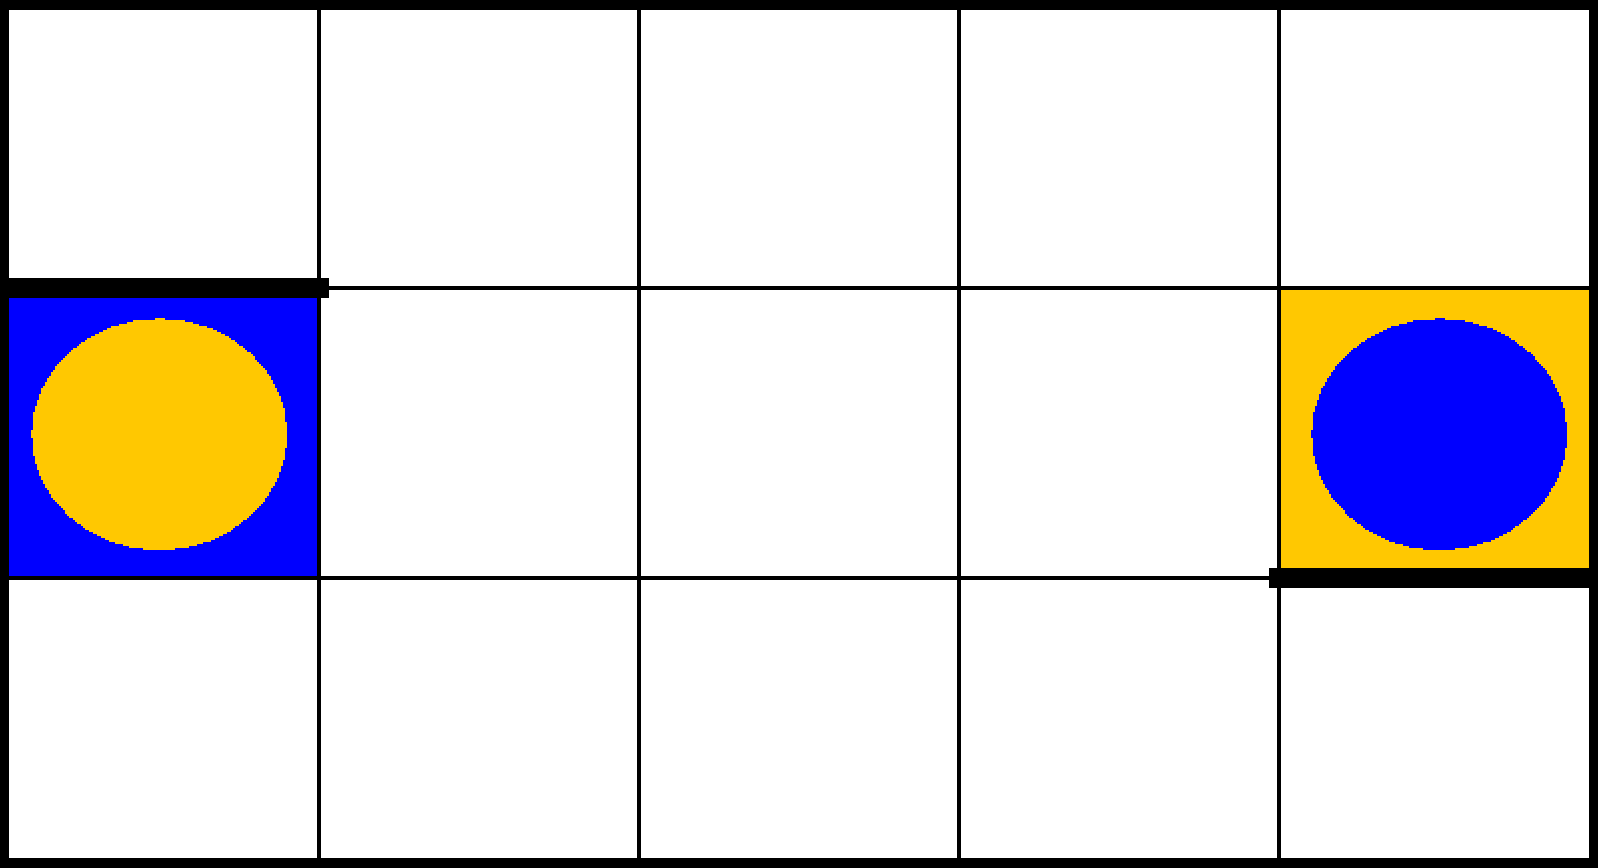
\includegraphics[width=0.8\columnwidth]{figures/threebyfivetwowalls.png}
\caption{A three by five grid world which requires both agents to sacrifice the best path to coordinate. The walls provide a suggestion each agents initial coordinating move to limit conflicts. Subsequent rounds allow one agent to take advantage of trusting agents by moving straight to the goal}
\label{fig:threebyfivetwowalls}
\end{figure}


\begin{figure}
\centering
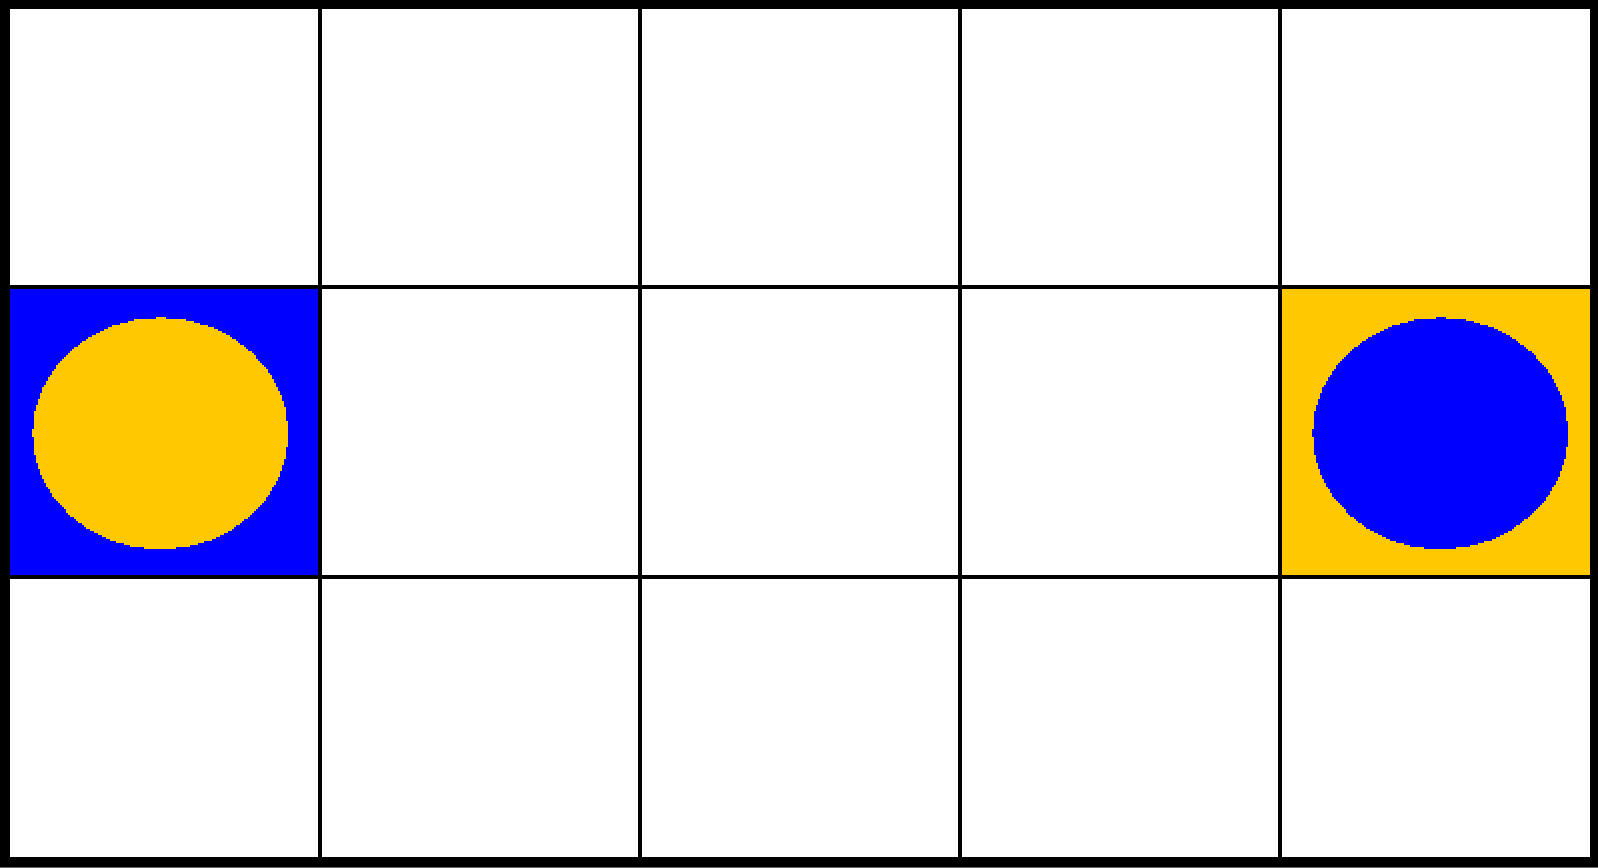
\includegraphics[width=0.8\columnwidth]{figures/threebyfive.png}
\caption{Three by five grid world which requires an agreed upon coordination to efficiently solve the game. Several coordination strategies also allow the agent to defend against an uncooperative partner without losing the game}
\label{fig:threebyfive}
\end{figure}

The grid world in figure~\ref{fig:threebyfivehallways} requires the blue agent to defend against an uncooperative orange agent by squatting on the orange goal. The orange agent should then move to $(3,3)$ where both agents are equidistant from their goals. This cooperative-defensive strategy requires more actions than a fully trusting strategy, where orange waits a single step before proceeding into its goal. However, blue does not have the opportunity to observe if orange will cooperate or defect and therefore cannot defend against orange should blue choose to move straight toward its goal.


\begin{figure}
\centering
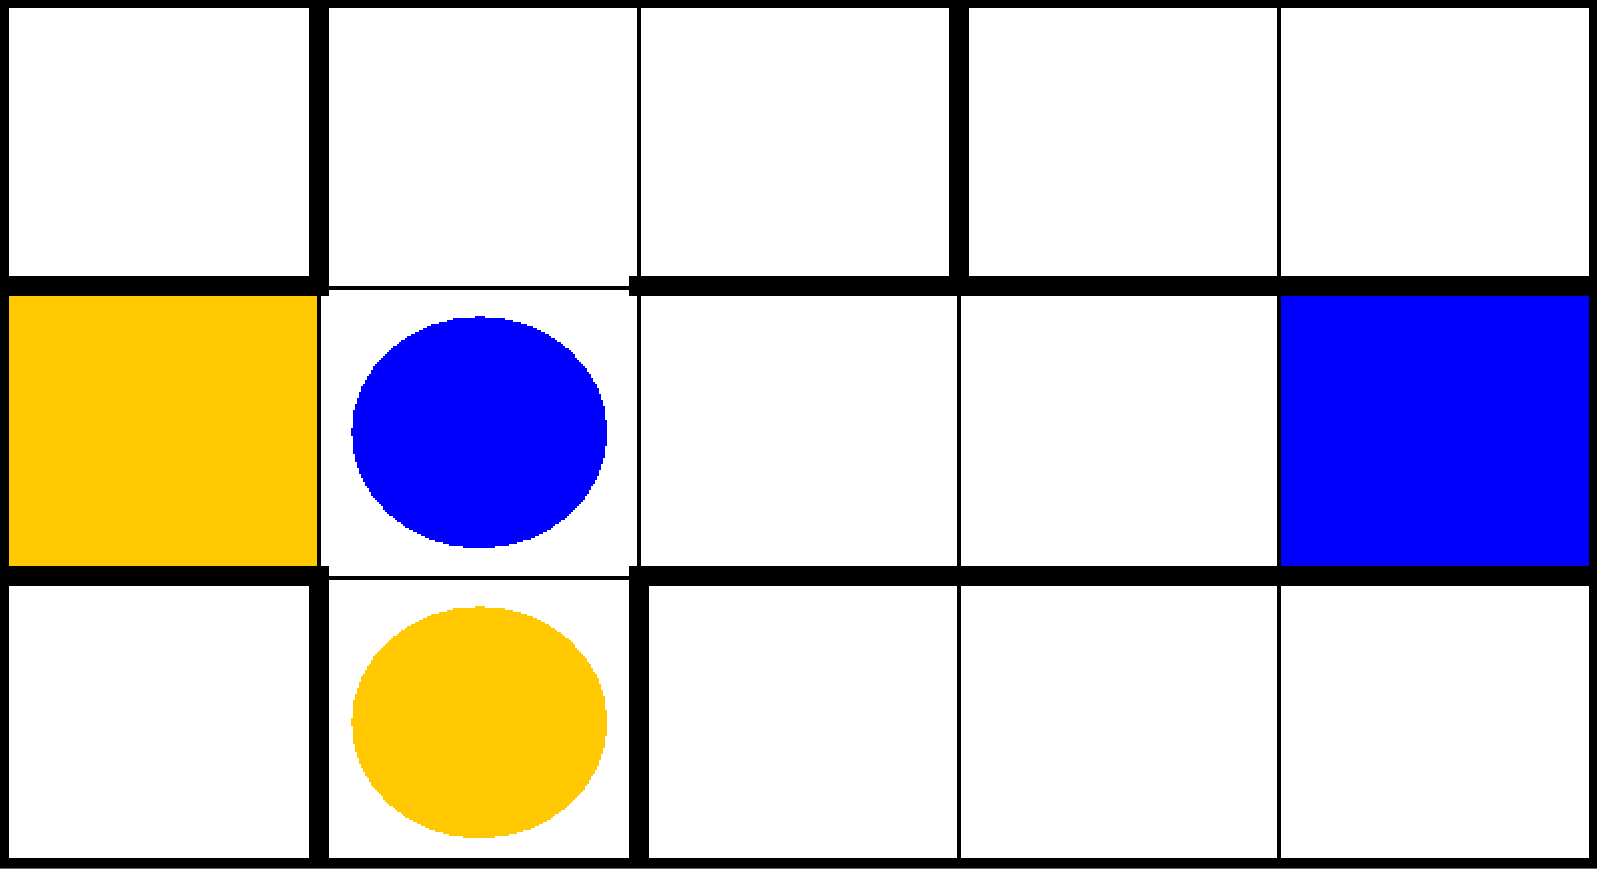
\includegraphics[width=0.8\columnwidth]{figures/threebyfivehallways.png}
\caption{Three by five grid world which requires blue to defend orange's goal to encourage orange to cooperate and move into the upmost hallway.}
\label{fig:threebyfivehallways}
\end{figure}

Figure~\ref{fig:threebyfivewindow} is a grid world that requires coordination to navigate through the center aisle at $(3,2)$. The best cooperative-defensive strategy is asymmetrical and requires one agent to cede to the other agent the center aisle. If agent chooses to cede the aisle, they should step west into $(2,1)$ while blue steps south into $(3,2)$. Then orange needs to step east back into $(3,1)$ to prevent blue from marching straight for the goal. Only when blue agrees to step into $(2,2)$ and orange ends up in $(3,1)$ will they both be equidistant from their respective goals.

\begin{figure}
\centering
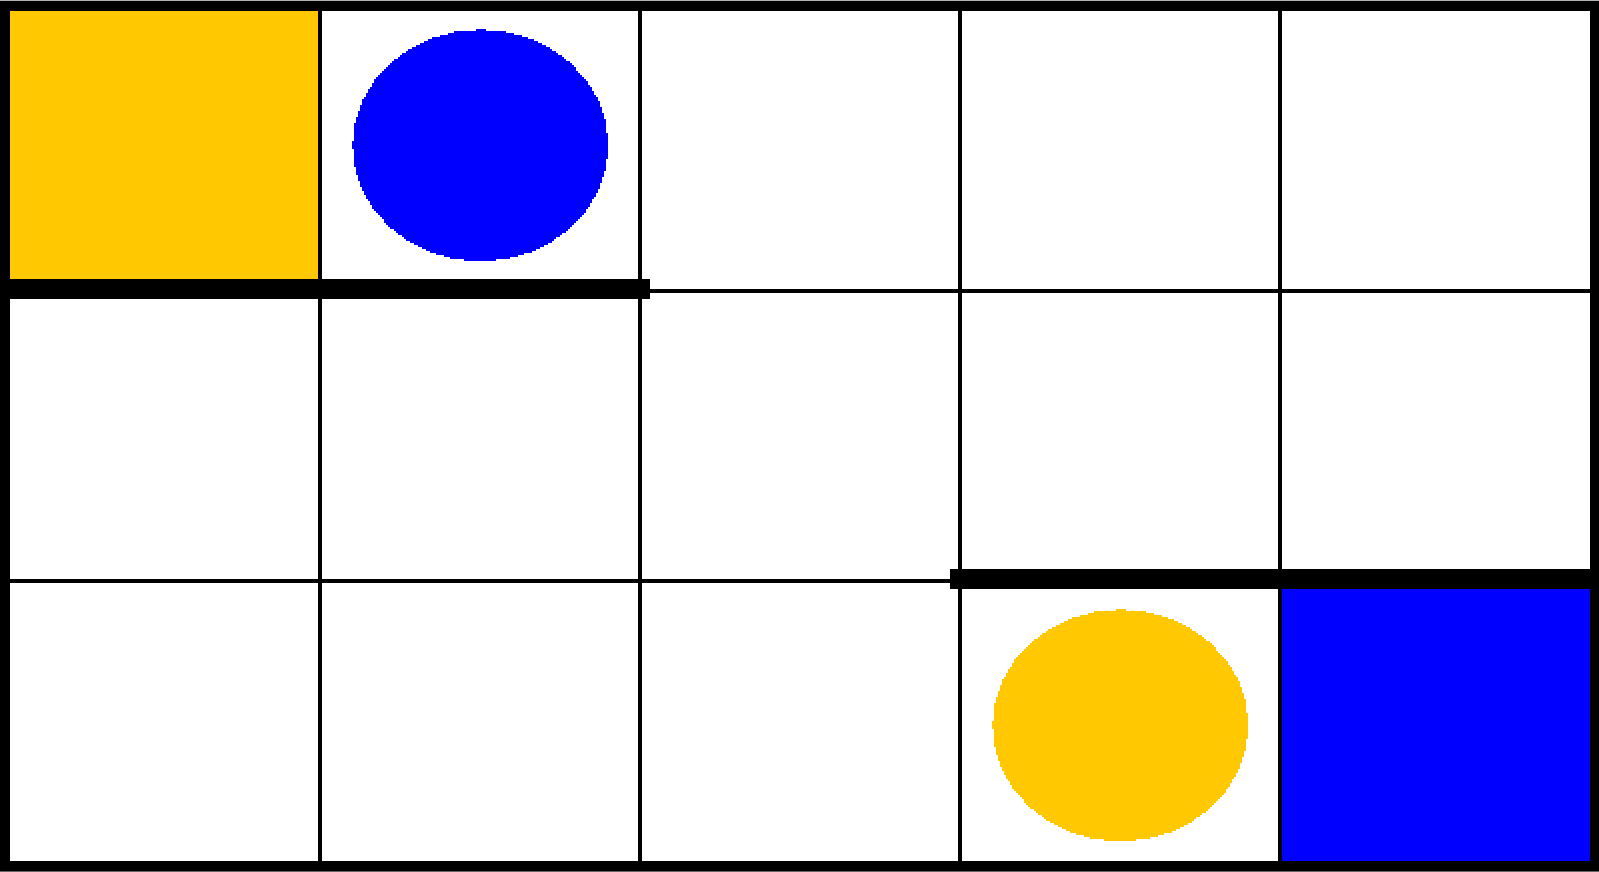
\includegraphics[width=0.8\columnwidth]{figures/threebyfivewindow.png}
\caption{A three by five grid world which requires the partners to trust and agree on an order to navigate through the window.}
\label{fig:threebyfivewindow}
\end{figure}





Long hall (figure~\ref{fig:longhallway}) begins with the blue agent one step closer to its goal than the orange. However, the orange agent can squat on the blue goal until the blue agent chooses to cooperate by stepping one square back. If the orange agent can predict when blue steps back, orange can pivot left and step one closer to the goal while blue attempts to step further away. The cooperative strategy that minimizes the risk to either requires the blue agent to wait one step initially, while the orange agent moves toward its goal.

\begin{figure}
\centering
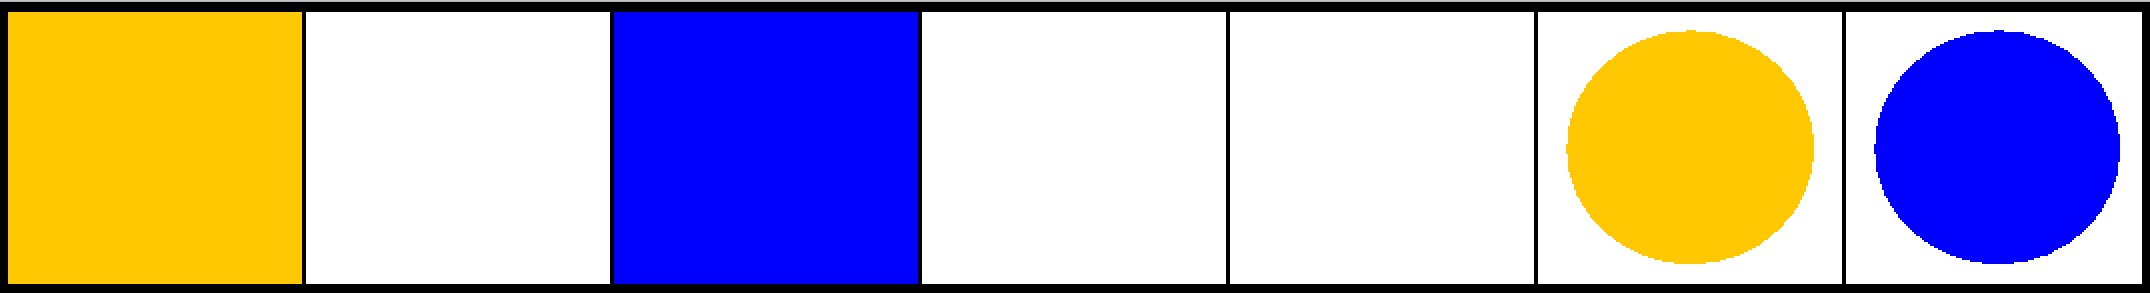
\includegraphics[width=0.8\columnwidth]{figures/longhallway.png}
\caption{Long Hall, A one by seven grid world which allows orange to squat on the blue agent's goal should they choose to not cooperate.}
\label{fig:longhallway}
\end{figure}

No Compromise (figure~\ref{fig:nocompromise}) requires both agents to trust and cooperate with each other in order to arrive at the goals at the same time. For example, the orange agent may sit on the blue agent's goal to let them pass into square $(1,2)$. Then the blue agent must wait two turns before both agents are equidistant from the goals. If the blue agent defects and moves north into $(1,1)$ while the orange agent moves south from $(2,1)$ into $(2,2)$, orange has the opportunity to step north to block blue from reaching the goal. However, if blue moves north into $(1,1)$ when orange steps east into $(3,2)$, blue will arrive at its goal sooner. Therefore a trust spanning multiple games is required for the agents to effectively solve a repetitive match.

\begin{figure}
\centering
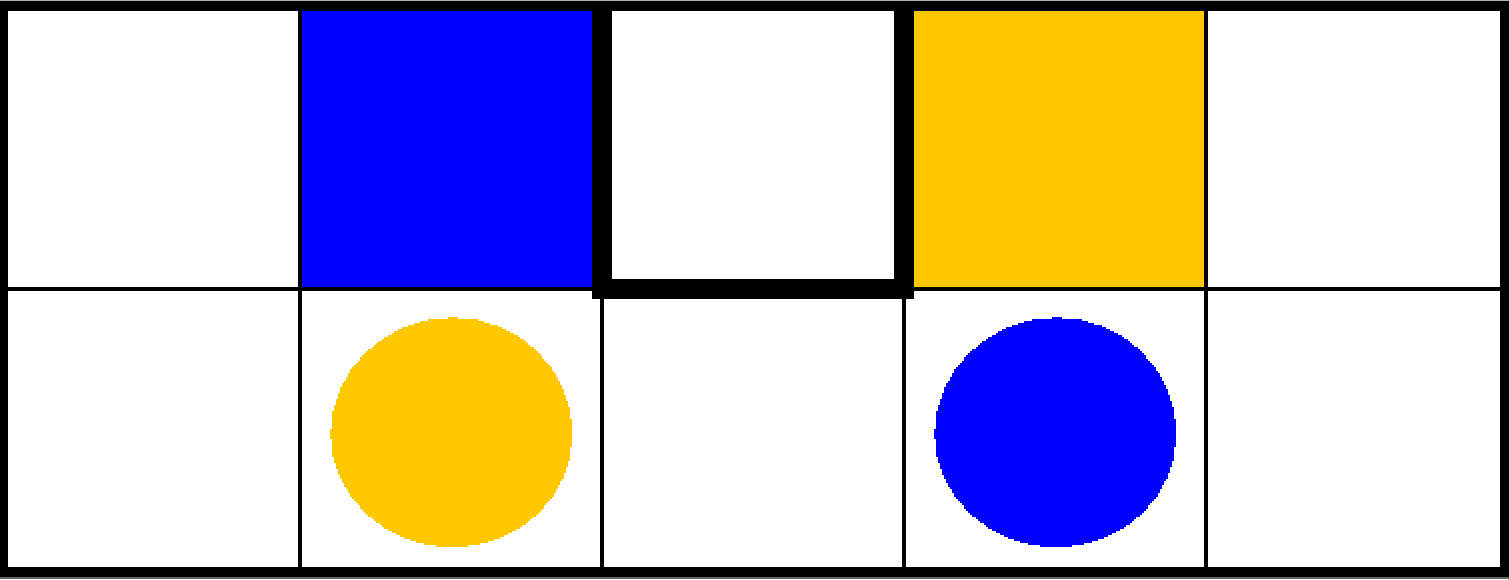
\includegraphics[width=0.8\columnwidth]{figures/nocompromise.png}
\caption{No Compromise, A two by five grid world which requires one agent to sit on the other's goal and then move to their goal when the other agent has passed}
\label{fig:nocompromise}
\end{figure}

\end{document}